\begin{enumerate}[label=\thesubsection.\arabic*, ref=\thesubsection.\theenumi]
    \item If $x = 3$ is one root of the quadratic equation $x^2 - 2kx - 6 = 0$, then find the value of $k$.

\solution Since $x = 3$ is a root of the given quadratic equation, from \eqref{eq:EE26BTECH11225-root}, substituting $x = 3$ into $x^2 - 2kx - 6 = 0$:
\begin{align}
    (3)^2 - 2k(3) - 6 &= 0 \\
    &\implies 9 - 6k - 6 = 0 \\
    &\implies 3 - 6k = 0 \\
    &\implies 6k = 3 
\end{align}
Thus, the value of $k$ is $\frac{1}{2}$.
    \item What is the HCF of smallest prime number and the smallest composite number?

\solution 
\begin{align}
    \text{Smallest prime number} &= 2 \\
    \text{Smallest composite number} &= 4
\end{align}
Expressing both as prime factors:
\begin{align}
    2 &= 2^1 \\
    4 &= 2^2 \\
    &\implies \text{HCF}(2, 4) = 2^1 = 2
\end{align}
    \item Find the distance of a point $P(x, y)$ from the origin.

\solution From \eqref{eq:EE26BTECH11225-distance}, the distance of $P(x, y)$ from $O(0, 0)$ is:
\begin{align}
    d &= \sqrt{(x - 0)^2 + (y - 0)^2} \\
    &= \sqrt{x^2 + y^2}
\end{align}
    \item In an AP, if the common difference $(d) = -4$, and the seventh term $(a_7)$ is 4, then find the first term.

\solution
The A.P. is the sequence $x(n)$ with first term $a$ and common difference $d = -4$. From \eqref{eq:EE26BTECH11225-ap-step},
\begin{align}
x(n) = \brak{a + (n-1)d}\,u(n-1) = \brak{a - 4(n-1)}\,u(n-1)
\end{align}
\par\noindent\hfill\mbox{\textit{(\ref{eq:EE26BTECH11225-ap-step})}}\par
Since $u(6) = 1$, the seventh term is $x(7) = a - 24$. Equating it to the given value,
\begin{align}
a - 24 = 4 \implies a = 28
\end{align}
The first term is therefore $\boxed{28}$. The C program prints the sequence, which the unit step switches on at $n = 1$, and the Python program plots it in \figref{fig:ap_q4}.
\begin{lstlisting}[frame=single, basicstyle=\rmfamily, escapeinside={(*@}{@*)}]
(*@\makebox[\dimexpr\linewidth-2\fboxsep-2\fboxrule\relax][c]{codes/1.2.4.c}@*)
\end{lstlisting}
\begin{lstlisting}[frame=single, basicstyle=\rmfamily, escapeinside={(*@}{@*)}]
(*@\makebox[\dimexpr\linewidth-2\fboxsep-2\fboxrule\relax][c]{codes/1.2.4.py}@*)
\end{lstlisting}
\begin{figure}[H]
    \centering
    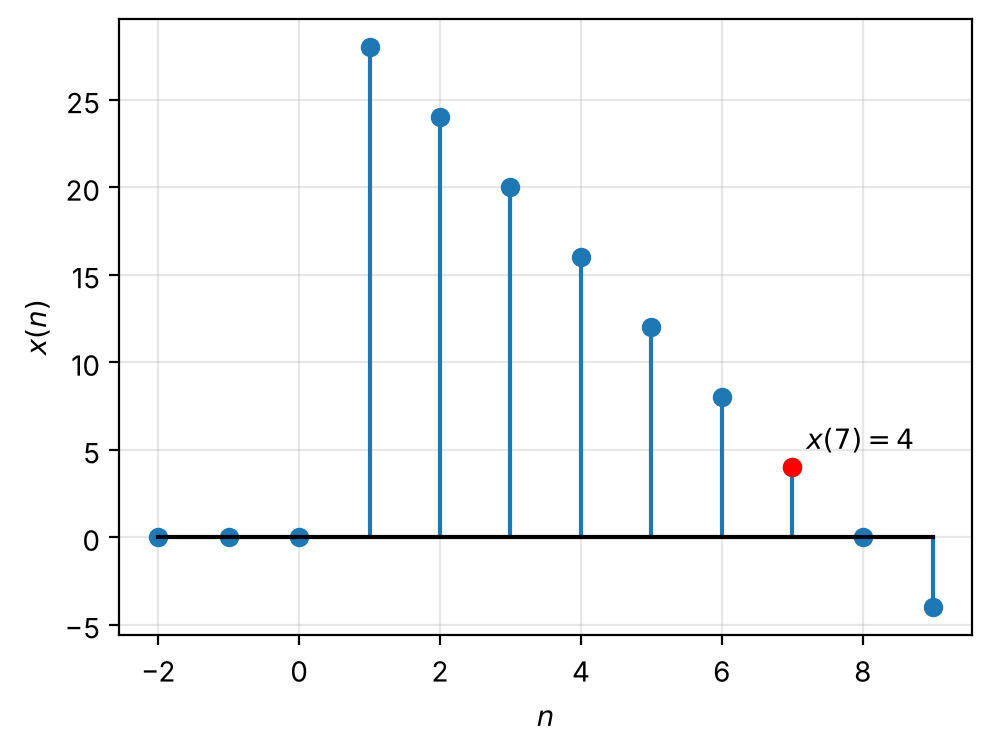
\includegraphics[width=0.65\linewidth]{figs/1.2.4.png}
    \caption{The A.P. as the sequence $x(n) = (a + (n-1)d)\,u(n-1)$}
    \label{fig:ap_q4}
\end{figure}

	\item What is the value of $(\cos^2 67^\circ - \sin^2 23^\circ)$?

\solution From \eqref{eq:EE26BTECH11225-complementary}, $\cos(90^\circ - \theta) = \sin \theta$:
\begin{align}
    \cos 67^\circ &= \cos(90^\circ - 23^\circ) \\
    &\implies \cos 67^\circ = \sin 23^\circ \\
    &\implies \cos^2 67^\circ - \sin^2 23^\circ = \sin^2 23^\circ - \sin^2 23^\circ = 0
\end{align}
    \item Given $\Delta ABC \sim \Delta PQR$, if $\frac{AB}{PQ} = \frac{1}{3}$, then find $\frac{\text{ar}(\Delta ABC)}{\text{ar}(\Delta PQR)}$.

\solution From \eqref{eq:EE26BTECH11225-area-ratio} (area ratio theorem for similar triangles):
\begin{align}
    \frac{\text{ar}(\Delta ABC)}{\text{ar}(\Delta PQR)} &= \left(\frac{AB}{PQ}\right)^2 \\
    &\implies \frac{\text{ar}(\Delta ABC)}{\text{ar}(\Delta PQR)} = \left(\frac{1}{3}\right)^2 = \frac{1}{9}
\end{align}
    \item Given that $\sqrt{2}$ is irrational, prove that $(5+3\sqrt{2})$ is an irrational number.

\solution Assume $(5+3\sqrt{2})$ is rational, so $5+3\sqrt{2} = \frac{a}{b}$ where $a, b \in \mathbb{Z}, b \neq 0$:
\begin{align}
    3\sqrt{2} &= \frac{a}{b} - 5 \\
    &\implies \sqrt{2} = \frac{a - 5b}{3b}
\end{align}
Since $a, b \in \mathbb{Z}$, the expression $\frac{a - 5b}{3b}$ is rational. This contradicts the given fact that $\sqrt{2}$ is irrational. Hence, $(5+3\sqrt{2})$ is irrational.

    \item In \figref{fig:rectangle_q8}, $ABCD$ is a rectangle. Find the values of $x$ and $y$.
    \begin{figure}[H]
\centering
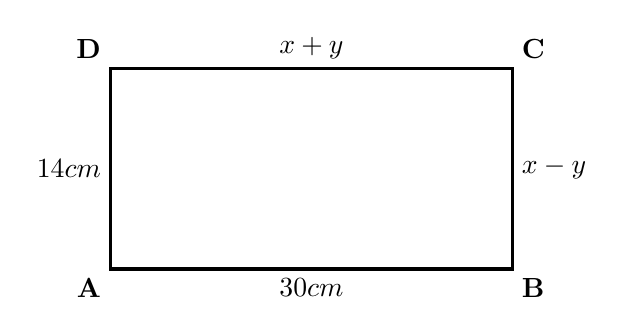
\begin{tikzpicture}[scale=0.85]
    % Draw the rectangle box (width 6, height 3)
    \draw[line width=1.2pt] (0,0) -- (6,0) -- (6,3) -- (0,3) -- cycle;

    % Vertex labels (A, B, C, D)
    \node[below left] at (0,0) {\textbf{A}};
    \node[below right] at (6,0) {\textbf{B}};
    \node[above right] at (6,3) {\textbf{C}};
    \node[above left] at (0,3) {\textbf{D}};

    % Side measurement labels
    \node[below] at (3, 0) {$30\text{ cm}$};
    \node[right] at (6, 1.5) {$x - y$};
    \node[above] at (3, 3) {$x + y$};
    \node[left] at (0, 1.5) {$14\text{ cm}$};
\end{tikzpicture}

\caption{Rectangle $ABCD$}
\label{fig:rectangle_q8}
\end{figure} 

\solution Opposite sides of a rectangle are equal in length.
\begin{align}
    x + y &= 30 \label{eq:EE26BTECH11225-rect-1} \\
    x - y &= 14 \label{eq:EE26BTECH11225-rect-2}
\end{align}
Adding \eqref{eq:EE26BTECH11225-rect-1} and \eqref{eq:EE26BTECH11225-rect-2}:
\begin{align}
    (x + y) + (x - y) &= 30 + 14 \\
    &\implies 2x = 44 \\
    &\implies x = 22
\end{align}
Substituting $x = 22$ into \eqref{eq:EE26BTECH11225-rect-1}:
\begin{align}
    22 + y &= 30 \\
    &\implies y = 30 - 22 \\
    &\implies y = 8
\end{align}
Thus, $x = 22$ and $y = 8$.
    \item Find the sum of first 8 multiples of 3.

\solution The first 8 multiples of 3 form an A.P.: $3, 6, 9, \dots$ with first term $a = 3$, common difference $d = 3$, and $n = 8$. From \eqref{eq:EE26BTECH11225-ap-sum},
\begin{align}
    S_n &= \frac{n}{2}[2a + (n-1)d] \\
    &\implies S_8 = \frac{8}{2}[2(3) + (8-1)3] \\
    &\implies S_8 = 4[6 + 21] \\
    &\implies S_8 = 4(27) = 108
\end{align}
    \item Find the ratio in which $P(4, m)$ divides the line segment joining the points $A(2, 3)$ and $B(6, -3)$. Hence find $m$.

\solution Let $P(4, m)$ divide $AB$ in the ratio $k : 1$. From \eqref{eq:EE26BTECH11225-section}, for the $x$-coordinate:
\begin{align}
    x &= \frac{k(x_2) + 1(x_1)}{k + 1} \\
    &\implies 4 = \frac{k(6) + 1(2)}{k + 1} \\
    &\implies 4(k + 1) = 6k + 2 \\
    &\implies 4k + 4 = 6k + 2 \\
    &\implies 2k = 2 \implies k = 1
\end{align}
Thus, the ratio is $1 : 1$. Now from \eqref{eq:EE26BTECH11225-section}, for the $y$-coordinate:
\begin{align}
    m &= \frac{1(-3) + 1(3)}{1 + 1} \\
    &\implies m = \frac{0}{2} = 0
\end{align}The following code verifies the result and generates \figref{fig:section_q10}.
\begin{lstlisting}[frame=single, basicstyle=\rmfamily, escapeinside={(*@}{@*)}]
(*@\makebox[\dimexpr\linewidth-2\fboxsep-2\fboxrule\relax][c]{codes/1.2.10.py}@*)
\end{lstlisting}
\begin{figure}[H]
    \centering
    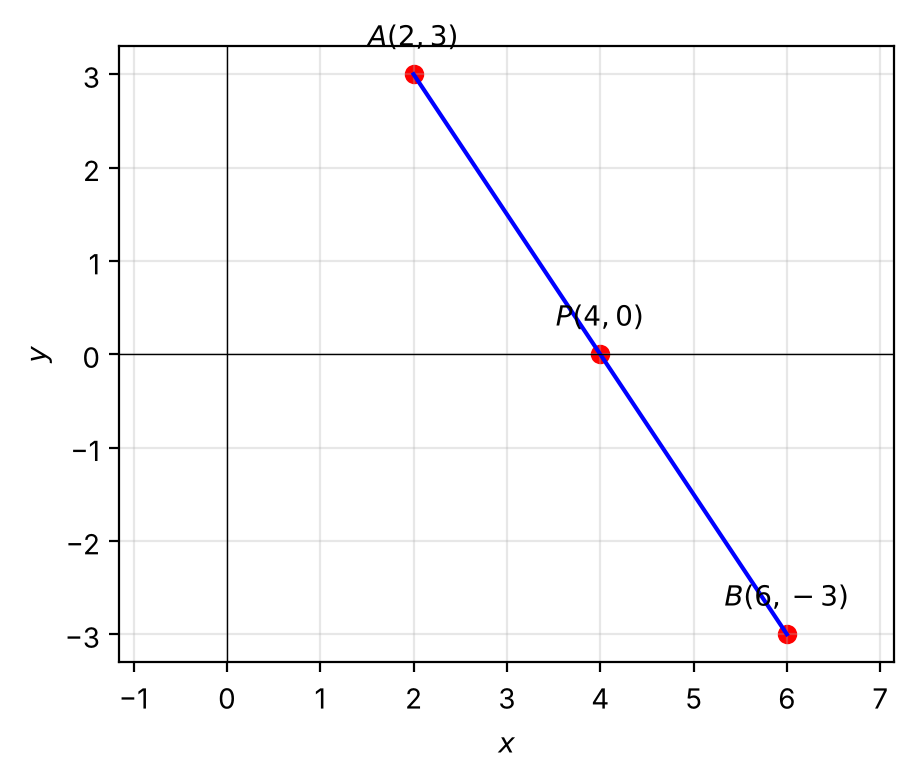
\includegraphics[width=0.60\linewidth]{figs/1.2.10.png}
    \caption{Point $P$ dividing $AB$}
    \label{fig:section_q10}
\end{figure}

    \item Two different dice are tossed together. Find the probability: \\[2pt]
(i) of getting a doublet. \\[2pt]
(ii) of getting a sum 10, of the numbers on the two dice.

\solution Let $X$ and $Y$ be the numbers on the two dice. They are independent and each is uniform on $\{1,\dots,6\}$, so from \eqref{eq:EE26BTECH11225-pmf-joint},
\begin{align}
    p_{XY}(i,j) = \frac{1}{6}\cdot\frac{1}{6} = \frac{1}{36}, \quad i,j \in \{1,\dots,6\}
\end{align}
(i) A doublet means $X = Y$. From \eqref{eq:EE26BTECH11225-pmf},
\begin{align}
    \Pr\brak{X = Y} = \sum_{i=1}^{6} p_{XY}(i,i) = 6 \cdot \frac{1}{36} = \frac{1}{6}
\end{align}
(ii) A sum of 10 means $(X,Y) \in \{(4,6),(5,5),(6,4)\}$:
\begin{align}
    \Pr\brak{X + Y = 10} = \sum_{i=4}^{6} p_{XY}(i,10-i) = 3 \cdot \frac{1}{36} = \frac{1}{12}
\end{align}
The following code builds the joint PMF of the two dice and verifies both probabilities.
\begin{lstlisting}[frame=single, basicstyle=\rmfamily, escapeinside={(*@}{@*)}]
(*@\makebox[\dimexpr\linewidth-2\fboxsep-2\fboxrule\relax][c]{codes/1.2.11.py}@*)
\end{lstlisting}

    \item An integer is chosen at random between 1 and 100. Find the probability that it is: \\[2pt]
(i) divisible by 8. \\[2pt]
(ii) not divisible by 8.

\solution Taking ``between $1$ and $100$'' to exclude both $1$ and $100$, the integer $X$ takes the values $2,3,\dots,99$, which are $98$ equally likely values. Its PMF is
\begin{align}
    p_X(k) = \frac{1}{98}, \quad k \in \{2,3,\dots,99\}
\end{align}
(i) The multiples of $8$ are $E = \{8,16,\dots,96\}$, which has $12$ values. From \eqref{eq:EE26BTECH11225-pmf},
\begin{align}
    \Pr\brak{8 \mid X} = \sum_{k \in E} p_X(k) = \frac{12}{98} = \frac{6}{49}
\end{align}
(ii) Since $\sum_k p_X(k) = 1$,
\begin{align}
    \Pr\brak{8 \nmid X} = 1 - \sum_{k \in E} p_X(k) = 1 - \frac{6}{49} = \frac{43}{49}
\end{align}
\item Find HCF and LCM of 404 and 96 and verify that $\text{HCF} \times \text{LCM} = \text{Product of the two given numbers}$.

\solution Expressing numbers as products of prime factors:
\begin{align}
    404 &= 2^2 \times 101 \\
    96 &= 2^5 \times 3 \\
    &\implies \text{HCF}(404, 96) = 2^2 = 4 \\
    &\implies \text{LCM}(404, 96) = 2^5 \times 3 \times 101 = 9696
\end{align}
Verification:
\begin{align}
    \text{LHS} &= \text{HCF} \times \text{LCM} = 4 \times 9696 = 38784 \\
    \text{RHS} &= 404 \times 96 = 38784 \\
    &\implies \text{LHS} = \text{RHS}
\end{align}
    \item Find all zeroes of the polynomial $(2x^4 - 9x^3 + 5x^2 + 3x - 1)$ if two of its zeroes are $(2+\sqrt{3})$ and $(2-\sqrt{3})$.

\solution Given zeroes $x = 2 \pm \sqrt{3}$, from \eqref{eq:EE26BTECH11225-factor}, $(x-\alpha)(x-\beta)$ is a factor of $p(x)$:
\begin{align}
    [x - (2 + \sqrt{3})][x - (2 - \sqrt{3})] &= (x - 2)^2 - 3 \\
    &= x^2 - 4x + 4 - 3 \\
    &\implies g(x) = x^2 - 4x + 1 \text{ is a factor}
\end{align}
Dividing $p(x) = 2x^4 - 9x^3 + 5x^2 + 3x - 1$ by $g(x) = x^2 - 4x + 1$:
\begin{align}
    2x^4 - 9x^3 + 5x^2 + 3x - 1 &= (x^2 - 4x + 1)(2x^2 - x - 1)
\end{align}
To find the remaining zeroes, set $2x^2 - x - 1 = 0$:
\begin{align}
    2x^2 - 2x + x - 1 &= 0 \\
    2x(x - 1) + 1(x - 1) &= 0 \\
    (2x + 1)(x - 1) &= 0 \\
    &\implies x = 1 \quad \text{or} \quad x = -\frac{1}{2}
\end{align}
Thus, all zeroes are $2+\sqrt{3}$, $2-\sqrt{3}$, $1$, and $-\frac{1}{2}$.The following code verifies the zeroes and plots $p(x)$ in \figref{fig:poly_q14}.
\begin{lstlisting}[frame=single, basicstyle=\rmfamily, escapeinside={(*@}{@*)}]
(*@\makebox[\dimexpr\linewidth-2\fboxsep-2\fboxrule\relax][c]{codes/1.2.14.py}@*)
\end{lstlisting}
\begin{figure}[H]
    \centering
    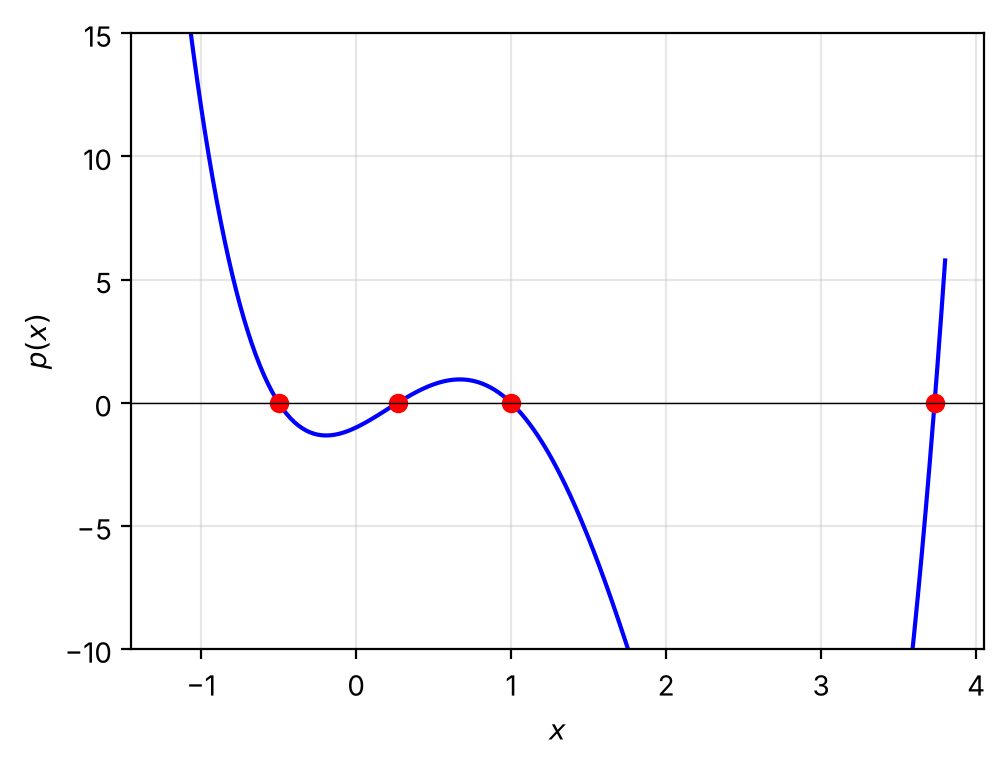
\includegraphics[width=0.70\linewidth]{figs/1.2.14.png}
    \caption{Plot of $p(x)=2x^4-9x^3+5x^2+3x-1$ with its zeroes}
    \label{fig:poly_q14}
\end{figure}

   \item 
    \begin{enumerate}[label=(\alph*), leftmargin=*, labelsep=0.5em]
        \item If $A(-2,1)$, $B(a,0)$, $C(4,b)$ and $D(1,2)$ are the vertices of a parallelogram $ABCD$, find the values of $a$ and $b$. Hence find the lengths of its sides.
        
        \begin{center}
            \textbf{OR}
        \end{center}
        
        \item If $A(-5,7)$, $B(-4,-5)$, $C(-1,-6)$ and $D(4,5)$ are the vertices of a quadrilateral, find the area of the quadrilateral $ABCD$.
    \end{enumerate} \vspace{2pt}
    \textbf{(a) Solution:} In a parallelogram, the diagonals bisect each other. Therefore, the midpoint of diagonal $AC$ is equal to the midpoint of diagonal $BD$.

From \eqref{eq:EE26BTECH11225-section} with $k=1$, the midpoint of $AC$ is:
\begin{align}
    M_{AC} &= \left( \frac{-2 + 4}{2}, \frac{1 + b}{2} \right) = \left( 1, \frac{1 + b}{2} \right)
\end{align}
Midpoint of $BD$:
\begin{align}
    M_{BD} &= \left( \frac{a + 1}{2}, \frac{0 + 2}{2} \right) = \left( \frac{a + 1}{2}, 1 \right)
\end{align}
Equating the $x$-coordinates and $y$-coordinates:
\begin{align}
    \frac{a + 1}{2} = 1 &\implies a + 1 = 2 \implies a = 1 \\
    \frac{1 + b}{2} = 1 &\implies 1 + b = 2 \implies b = 1
\end{align}
Thus, the vertices are $A(-2,1)$, $B(1,0)$, $C(4,1)$, and $D(1,2)$. \\[4pt]
Now, from \eqref{eq:EE26BTECH11225-distance}, the lengths of the sides are:
\begin{align}
    AB &= \sqrt{(1 - (-2))^2 + (0 - 1)^2} = \sqrt{3^2 + (-1)^2} = \sqrt{9 + 1} = \sqrt{10} \\
    BC &= \sqrt{(4 - 1)^2 + (1 - 0)^2} = \sqrt{3^2 + 1^2} = \sqrt{9 + 1} = \sqrt{10}
\end{align}
Since opposite sides of a parallelogram are equal:
\begin{align}
    CD &= AB = \sqrt{10} \\
    AD &= BC = \sqrt{10}
\end{align}
Thus, $a = 1, b = 1$, and all four sides have length $\sqrt{10}$ units. \\[8pt]
\textbf{(b) Solution:} Joining diagonal $AC$ divides quadrilateral $ABCD$ into two triangles: $\Delta ABC$ and $\Delta ADC$.

From \eqref{eq:EE26BTECH11225-area-triangle}, the area of a triangle with vertices $(x_1,y_1), (x_2,y_2), (x_3,y_3)$ is given by:
\begin{align}
    \text{Area} &= \frac{1}{2} \big| x_1(y_2 - y_3) + x_2(y_3 - y_1) + x_3(y_1 - y_2) \big|
\end{align}

For $\Delta ABC$ with $A(-5,7)$, $B(-4,-5)$, and $C(-1,-6)$:
\begin{align}
    \text{Area}(\Delta ABC) &= \frac{1}{2} \big| -5(-5 - (-6)) + (-4)(-6 - 7) + (-1)(7 - (-5)) \big| \\
    &= \frac{1}{2} \big| -5(1) + (-4)(-13) + (-1)(12) \big| \\
    &= \frac{1}{2} \big| -5 + 52 - 12 \big| \\
    &= \frac{1}{2} |35| = 17.5\text{ sq. units}
\end{align}

For $\Delta ADC$ with $A(-5,7)$, $D(4,5)$, and $C(-1,-6)$:
\begin{align}
    \text{Area}(\Delta ADC) &= \frac{1}{2} \big| -5(5 - (-6)) + 4(-6 - 7) + (-1)(7 - 5) \big| \\
    &= \frac{1}{2} \big| -5(11) + 4(-13) + (-1)(2) \big| \\
    &= \frac{1}{2} \big| -55 - 52 - 2 \big| \\
    &= \frac{1}{2} |-109| = 54.5\text{ sq. units}
\end{align}

From \eqref{eq:EE26BTECH11225-area-quad}, the total area of quadrilateral $ABCD$ is:
\begin{align}
    \text{Area}(ABCD) &= \text{Area}(\Delta ABC) + \text{Area}(\Delta ADC) \\
    &= 17.5 + 54.5 = 72\text{ sq. units}
\end{align}
Thus, the area of quadrilateral $ABCD$ is $72\text{ sq. units}$.The following code verifies both parts and generates \figref{fig:quad_q15}.
\begin{lstlisting}[frame=single, basicstyle=\rmfamily, escapeinside={(*@}{@*)}]
(*@\makebox[\dimexpr\linewidth-2\fboxsep-2\fboxrule\relax][c]{codes/1.2.15.py}@*)
\end{lstlisting}
\begin{figure}[H]
    \centering
    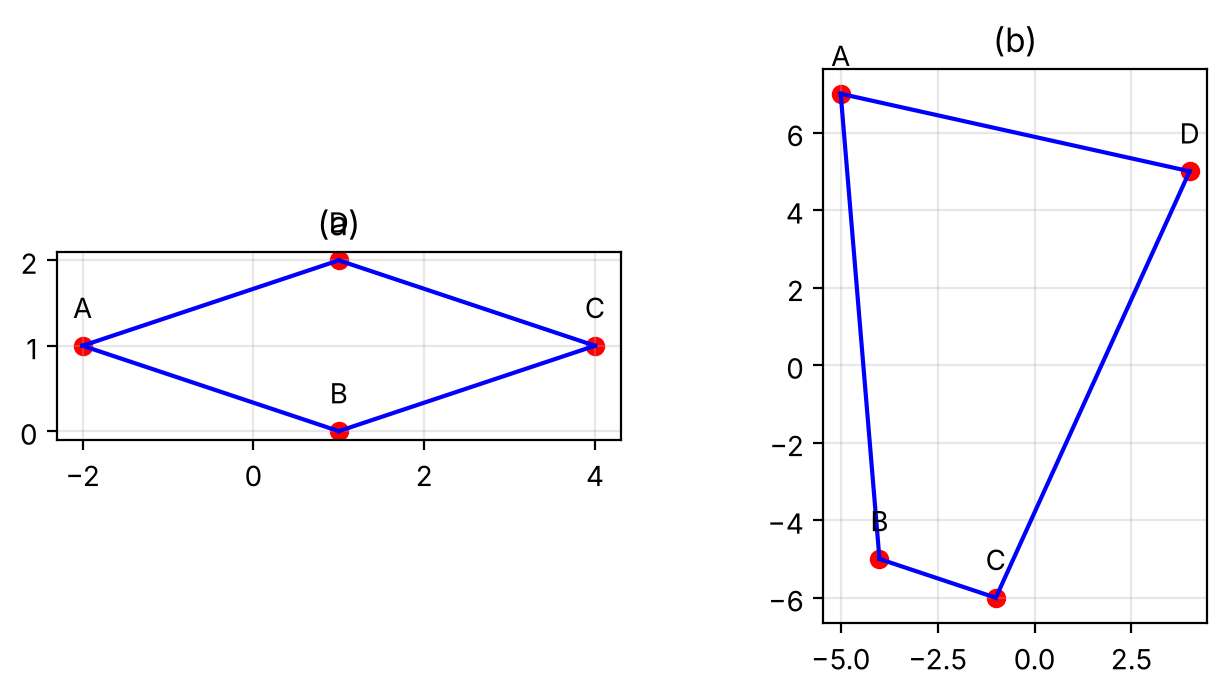
\includegraphics[width=0.95\linewidth]{figs/1.2.15.png}
    \caption{(a) Parallelogram $ABCD$ and (b) quadrilateral $ABCD$}
    \label{fig:quad_q15}
\end{figure}

    \item A plane left 30 minutes late than its scheduled time and in order to reach the destination 1500 km away in time, it had to increase its speed by 100 km/h from the usual speed. Find its usual speed.

\solution
Let the usual speed be $x$ km/h. The delay of $\frac{1}{2}$ hour on $1500$ km gives
\begin{align}
\frac{1500}{x} - \frac{1500}{x+100} = \frac{1}{2} \implies f(x) = x^2 + 100x - 300000 = 0
\end{align}
The speed is the positive root of $f$. With $f'(x) = 2x + 100$, the Newton--Raphson iteration is
\begin{align}
x_{n+1} = x_n - \frac{x_n^2 + 100x_n - 300000}{2x_n + 100}
\end{align}
\par\noindent\hfill\mbox{\textit{(\ref{eq:EE26BTECH11225-newton})}}\par
Starting from $x_0 = 1000$ and from $x_0 = -1000$, the C program gives
\[
\begin{array}{c|r|r}
n & x_n\;(x_0=1000) & x_n\;(x_0=-1000)\\\hline
0 & 1000.000000 & -1000.000000 \\
1 & 619.047619 & -684.210526 \\
2 & 510.591425 & -605.590740 \\
3 & 500.100054 & -600.028129 \\
4 & 500.000009 & -600.000001 \\
5 & 500.000000 & -600.000000 \\
6 & 500.000000 & -600.000000
\end{array}
\]
The iterates settle at $500$ and $-600$. Speed cannot be negative, so the usual speed is $\boxed{500\text{ km/h}}$. This agrees with $f(x) = (x-500)(x+600)$. The C program prints the iterates and checks both roots, and the Python program draws the first three Newton steps as tangent lines using CoordGeo in \figref{fig:newton_q16}.
\begin{lstlisting}[frame=single, basicstyle=\rmfamily, escapeinside={(*@}{@*)}]
(*@\makebox[\dimexpr\linewidth-2\fboxsep-2\fboxrule\relax][c]{codes/1.2.16.c}@*)
\end{lstlisting}
\begin{lstlisting}[frame=single, basicstyle=\rmfamily, escapeinside={(*@}{@*)}]
(*@\makebox[\dimexpr\linewidth-2\fboxsep-2\fboxrule\relax][c]{codes/1.2.16.py}@*)
\end{lstlisting}
\begin{figure}[H]
    \centering
    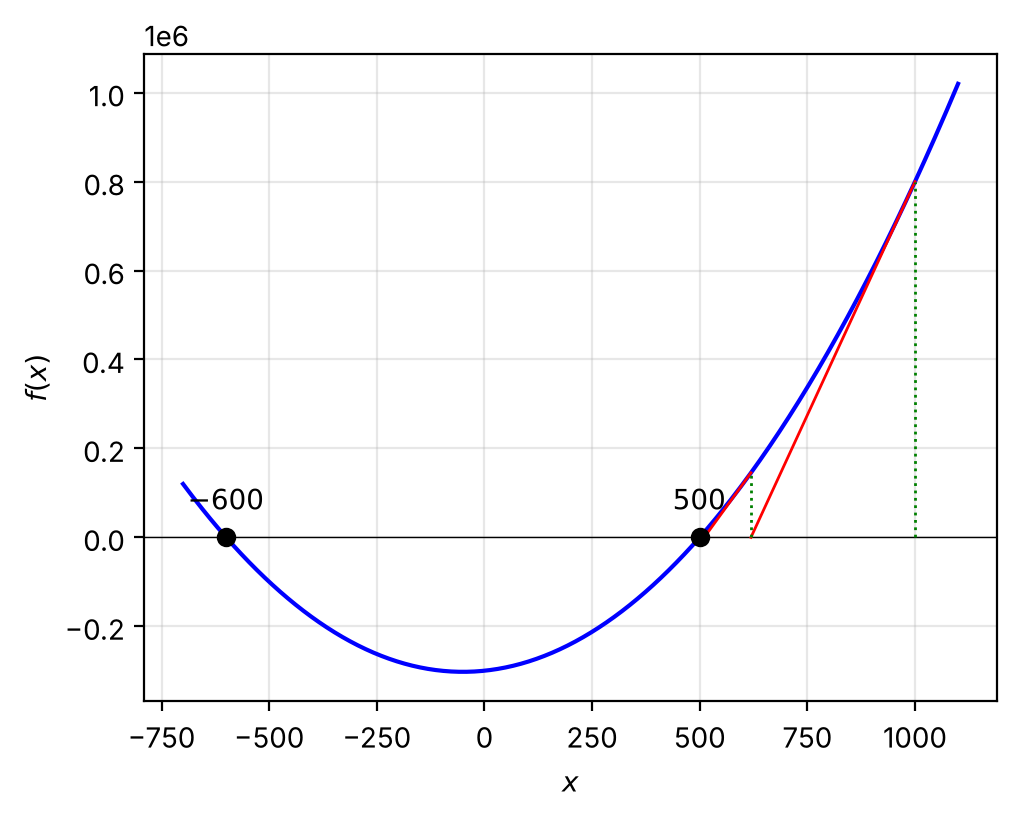
\includegraphics[width=0.65\linewidth]{figs/1.2.16.png}
    \caption{Newton--Raphson steps for $f(x) = x^2 + 100x - 300000$ from $x_0 = 1000$}
    \label{fig:newton_q16}
\end{figure}

    \item 
    \begin{enumerate}[label=(\alph*), leftmargin=1.5em, labelsep=0.5em]
        \item Prove that the area of an equilateral triangle described on one side of a square is equal to half the area of the equilateral triangle described on one of its diagonals.
        
        \vspace{0.5em}
        \begin{center}
            \textbf{OR}
        \end{center}
        \vspace{0.5em}

        \item If the areas of two similar triangles are equal, prove that they are congruent.	\\[2pt]
    \end{enumerate}
    \noindent\textbf{(a) Solution:} Let $ABCD$ be a square of side length $a$.
From \eqref{eq:EE26BTECH11225-pythagoras}, the length of diagonal $AC$ is given by:
\begin{align}
    AC &= \sqrt{a^2 + a^2} = a\sqrt{2}
\end{align}

\begin{center}
    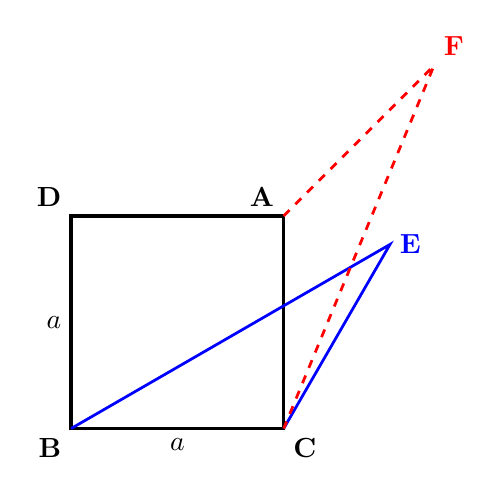
\begin{tikzpicture}[scale=0.9]
        % Square ABCD
        \draw[line width=1.2pt] (0,0) coordinate (B) -- (3,0) coordinate (C) -- (3,3) coordinate (A) -- (0,3) coordinate (D) -- cycle;
        
        % Diagonal AC
        \draw[thick, dashed] (A) -- (C);
        
        % Equilateral Triangle on side BC (BCE)
        \coordinate (E) at (4.5, 2.598);
        \draw[line width=1pt, blue] (B) -- (E) -- (C);
        
        % Equilateral Triangle on diagonal AC (ACF)
        % Angle of AC is -45 deg, side is 3*sqrt(2) = 4.242
        \coordinate (F) at (5.121, 5.121);
        \draw[line width=1pt, red, dashed] (A) -- (F) -- (C);
        
        % Labels
        \node[above left] at (D) {\textbf{D}};
        \node[above left] at (A) {\textbf{A}};
        \node[below left] at (B) {\textbf{B}};
        \node[below right] at (C) {\textbf{C}};
        \node[right, blue] at (E) {\textbf{E}};
        \node[above right, red] at (F) {\textbf{F}};
        
        % Side labels
        \node[below] at (1.5,0) {$a$};
        \node[left] at (0,1.5) {$a$};
    \end{tikzpicture}

    \captionof{figure}{Equilateral triangles $\Delta BCE$ on side $a$ and $\Delta ACF$ on diagonal $a\sqrt{2}$}
    \label{fig:square_triangles_q17}
\end{center} \vspace{2pt}

Let $\Delta BCE$ be the equilateral triangle described on side $BC = a$, and $\Delta ACF$ be the equilateral triangle described on diagonal $AC = a\sqrt{2}$.

Area of an equilateral triangle with side $s$ is given by $\frac{\sqrt{3}}{4} s^2$.

Area of $\Delta BCE$:
\begin{align}
    \text{Area}(\Delta BCE) &= \frac{\sqrt{3}}{4} a^2
\end{align}

Area of $\Delta ACF$:
\begin{align}
    \text{Area}(\Delta ACF) &= \frac{\sqrt{3}}{4} (a\sqrt{2})^2 = \frac{\sqrt{3}}{4} (2a^2) = 2 \left( \frac{\sqrt{3}}{4} a^2 \right) \\
    &\implies \text{Area}(\Delta BCE) = \frac{1}{2} \text{Area}(\Delta ACF)
\end{align}
Hence proved. \\[8pt]
\noindent\textbf{(b) Solution:} Let $\Delta ABC \sim \Delta PQR$ such that $\text{Area}(\Delta ABC) = \text{Area}(\Delta PQR)$.

From \eqref{eq:EE26BTECH11225-area-ratio} (area ratio theorem for similar triangles):
\begin{align}
    \frac{\text{Area}(\Delta ABC)}{\text{Area}(\Delta PQR)} &= \left(\frac{AB}{PQ}\right)^2 = \left(\frac{BC}{QR}\right)^2 = \left(\frac{AC}{PR}\right)^2
\end{align}

Since $\text{Area}(\Delta ABC) = \text{Area}(\Delta PQR)$, the ratio of their areas is $1$:
\begin{align}
    1 = \left(\frac{AB}{PQ}\right)^2 &\implies \frac{AB}{PQ} = 1 \implies AB = PQ \\
    1 = \left(\frac{BC}{QR}\right)^2 &\implies \frac{BC}{QR} = 1 \implies BC = QR \\
    1 = \left(\frac{AC}{PR}\right)^2 &\implies \frac{AC}{PR} = 1 \implies AC = PR
\end{align}

Since all three corresponding sides are equal ($AB = PQ$, $BC = QR$, $AC = PR$), by SSS congruence criterion:
\begin{align}
    \Delta ABC \cong \Delta PQR
\end{align}
Hence proved.
    \item Prove that the lengths of tangents drawn from an external point to a circle are equal.

\solution Let $P$ be an external point to a circle with centre $O$. Let $PA$ and $PB$ be two tangents drawn from $P$ touching the circle at points $A$ and $B$ respectively. Join $OA$, $OB$, and $OP$.

\begin{figure}[H]
    \centering
    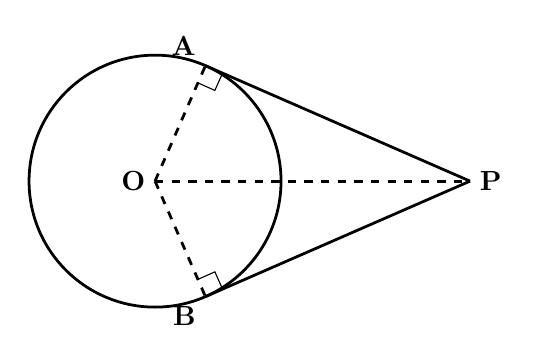
\begin{tikzpicture}[scale=0.8]
        % Circle centre and radius
        \coordinate (O) at (0,0);
        \draw[line width=1pt] (O) circle (2cm);
        
        % External point P
        \coordinate (P) at (5,0);
        
        % Tangent points A and B
        \coordinate (A) at (0.8, 1.833);
        \coordinate (B) at (0.8, -1.833);
        
        % Draw radius lines
        \draw[line width=1pt, dashed] (O) -- (A);
        \draw[line width=1pt, dashed] (O) -- (B);
        \draw[line width=1pt, dashed] (O) -- (P);
        
        % Draw tangent lines
        \draw[line width=1pt] (P) -- (A);
        \draw[line width=1pt] (P) -- (B);
        
        % Right angle indicators
        \draw (0.68, 1.56) -- (0.95, 1.44) -- (1.07, 1.71);
        \draw (0.68, -1.56) -- (0.95, -1.44) -- (1.07, -1.71);
        
        % Labels
        \node[left] at (O) {\textbf{O}};
        \node[right] at (P) {\textbf{P}};
        \node[above left] at (A) {\textbf{A}};
        \node[below left] at (B) {\textbf{B}};
    \end{tikzpicture}

    \caption{Tangents $PA$ and $PB$ from external point $P$ to circle with centre $O$}
    \label{fig:tangents_circle}
\end{figure}

In $\Delta OAP$ and $\Delta OBP$:
\begin{align}
    \angle OAP = \angle OBP &= 90^\circ \quad (\text{Radius is perpendicular to tangent, from } \eqref{eq:EE26BTECH11225-tangent-perp}) \\
    OP &= OP \quad (\text{Common hypotenuse}) \\
    OA &= OB \quad (\text{Radii of the same circle})
\end{align}
By RHS congruence criterion:
\begin{align}
    \Delta OAP \cong \Delta OBP &\implies PA = PB
\end{align}
Hence, the lengths of tangents drawn from an external point to a circle are equal.
    \item 
    \begin{enumerate}[label=(\alph*), leftmargin=1.5em, labelsep=0.5em]
        \item If $4 \tan\theta = 3$, evaluate $\left( \frac{4 \sin\theta - \cos\theta + 1}{4 \sin\theta + \cos\theta - 1} \right)$.
        
        \vspace{0.5em}
        \begin{center}
            \textbf{OR}
        \end{center}
        \vspace{0.5em}

        \item If $\tan 2A = \cot(A - 18^\circ)$, where $2A$ is an acute angle, find the value of $A$.	\\[2pt]
        \noindent\textbf{(a) Solution:} Given $4\tan\theta = 3 \implies \tan\theta = \frac{3}{4}$.

Consider a right-angled triangle with opposite side $= 3$ and adjacent side $= 4$.
By Pythagoras theorem, from \eqref{eq:EE26BTECH11225-pythagoras}, the hypotenuse is:
\begin{align}
    \text{Hypotenuse} &= \sqrt{3^2 + 4^2} = \sqrt{9 + 16} = \sqrt{25} = 5
\end{align}

Therefore, from \eqref{eq:EE26BTECH11225-trig-ratios}:
\begin{align}
    \sin\theta &= \frac{3}{5}, \quad \cos\theta = \frac{4}{5}
\end{align}

Substituting these values into the given expression:
\begin{align}
    \frac{4\sin\theta - \cos\theta + 1}{4\sin\theta + \cos\theta - 1} &= \frac{4\left(\frac{3}{5}\right) - \frac{4}{5} + 1}{4\left(\frac{3}{5}\right) + \frac{4}{5} - 1} \\
    &= \frac{\frac{12}{5} - \frac{4}{5} + 1}{\frac{12}{5} + \frac{4}{5} - 1} \\
    &= \frac{\frac{8}{5} + 1}{\frac{16}{5} - 1} \\
    &= \frac{\frac{13}{5}}{\frac{11}{5}} = \frac{13}{11}
\end{align}
Thus, the value of the expression is $\frac{13}{11}$. \\[8pt]
\noindent\textbf{(b) Solution:} Given $\tan 2A = \cot(A - 18^\circ)$.

From \eqref{eq:EE26BTECH11225-complementary}, $\tan \theta = \cot(90^\circ - \theta)$:
\begin{align}
    \cot(90^\circ - 2A) &= \cot(A - 18^\circ)
\end{align}

Equating the angles:
\begin{align}
    90^\circ - 2A &= A - 18^\circ \\
    &\implies 90^\circ + 18^\circ = A + 2A \\
    &\implies 3A = 108^\circ \\
    &\implies A = \frac{108^\circ}{3} = 36^\circ
\end{align}
Thus, the value of $A$ is $36^\circ$.
        
    \end{enumerate}
   \item Find the area of the shaded region in \figref{fig:shaded_q20}, where arcs drawn with centres $A, B, C$ and $D$ intersect in pairs at mid-points $P, Q, R$ and $S$ of the sides $AB, BC, CD$ and $DA$ respectively of a square $ABCD$ of side $12\text{ cm}$. [Use $\pi = 3.14$]

\begin{figure}[H]
\centering
\begin{tikzpicture}[scale=0.35]
    % Coordinates of Square Vertices
    \coordinate (A) at (0, 12);
    \coordinate (B) at (12, 12);
    \coordinate (C) at (12, 0);
    \coordinate (D) at (0, 0);

    % Midpoints
    \coordinate (P) at (6, 12);
    \coordinate (Q) at (12, 6);
    \coordinate (R) at (6, 0);
    \coordinate (S) at (0, 6);

    % Fill Shaded Region (Square minus 4 quadrant arcs)
    \begin{scope}
        \clip (A) -- (B) -- (C) -- (D) -- cycle;
        % Fill the full square first with pattern/color
        \fill[pattern=north east lines, pattern color=black!70] (A) -- (B) -- (C) -- (D) -- cycle;
        
        % Un-clip/white-out the 4 corner circular quadrants
        \fill[white] (A) -- (P) arc (0:-90:6) -- cycle;
        \fill[white] (B) -- (Q) arc (-90:-180:6) -- cycle;
        \fill[white] (C) -- (R) arc (180:90:6) -- cycle;
        \fill[white] (D) -- (S) arc (90:0:6) -- cycle;
    \end{scope}

    % Draw Outer Square
    \draw[line width=1.2pt] (A) -- (B) -- (C) -- (D) -- cycle;

    % Draw Arcs
    \draw[line width=1pt] (P) arc (0:-90:6);
    \draw[line width=1pt] (Q) arc (-90:-180:6);
    \draw[line width=1pt] (R) arc (180:90:6);
    \draw[line width=1pt] (S) arc (90:0:6);

    % Label Vertices
    \node[above left] at (A) {\textbf{A}};
    \node[above right] at (B) {\textbf{B}};
    \node[below right] at (C) {\textbf{C}};
    \node[below left] at (D) {\textbf{D}};

    % Label Midpoints
    \node[above] at (P) {\textbf{P}};
    \node[right] at (Q) {\textbf{Q}};
    \node[below] at (R) {\textbf{R}};
    \node[left] at (S) {\textbf{S}};
\end{tikzpicture}

\caption{Shaded region enclosed by circular arcs in square $ABCD$}
\label{fig:shaded_q20}
\end{figure}		 \vspace{2pt}


\solution Given:
\begin{align}
    \text{Side of square } ABCD \ (s) &= 12\text{ cm}
\end{align}

Since $P, Q, R, S$ are the mid-points of the sides of the square, the radius $r$ of each corner sector is:
\begin{align}
    r &= \frac{12}{2} = 6\text{ cm}
\end{align}

Each corner sector has an angle of $90^\circ$ (since all interior angles of a square are $90^\circ$), making each sector a quadrant of a circle. 

From \eqref{eq:EE26BTECH11225-sector}, combining these $4$ identical quadrants forms $1$ complete circle of radius $r = 6\text{ cm}$:
\begin{align}
    \text{Area of } 4\text{ quadrants} &= \text{Area of } 1\text{ full circle} = \pi r^2 \\
    &= 3.14 \times (6)^2 = 3.14 \times 36 = 113.04\text{ cm}^2
\end{align}

Calculating the area of the square:
\begin{align}
    \text{Area of square } ABCD &= s^2 = (12)^2 = 144\text{ cm}^2
\end{align}

Subtracting the area of the circle from the area of the square gives the area of the shaded region:
\begin{align}
    \text{Area of shaded region} &= \text{Area of square } ABCD - \text{Area of } 4\text{ quadrants} \\
    &= 144 - 113.04 = 30.96\text{ cm}^2
\end{align}

Thus, the area of the shaded region is $30.96\text{ cm}^2$.
	\item 
    \begin{enumerate}[label=(\alph*), leftmargin=1.5em, labelsep=0.5em]
        \item A wooden article was made by scooping out a hemisphere from each end of a solid cylinder, as shown in \figref{fig:wooden_q21}. If the height of the cylinder is $10\text{ cm}$ and its base is of radius $3.5\text{ cm}$, find the total surface area of the article.
        
        \begin{figure}[H]
            \centering
            \begin{tikzpicture}[scale=0.8]
            % Top Scooped Hemisphere Pattern Shading
            \path[pattern=north east lines, pattern color=black!70] 
                (-1.5, 2) arc (180:360:1.5 and 1.5) 
                arc (0:180:1.5 and 0.5) -- cycle;

            % Bottom Scooped Hemisphere Pattern Shading
            \path[pattern=north east lines, pattern color=black!70] 
                (-1.5, -2) arc (180:0:1.5 and 1.5) 
                arc (360:180:1.5 and 0.5) -- cycle;

            % Main Cylinder Body Outline
            \draw[thick] (-1.5, -2) -- (-1.5, 2);
            \draw[thick] (1.5, -2) -- (1.5, 2);
            
            % Top Cylinder Rim
            \draw[thick] (0, 2) ellipse (1.5 and 0.5);
            
            % Bottom Cylinder Rim
            \draw[thick] (0, -2) ellipse (1.5 and 0.5);
            
            % Top Scooped Hemisphere Arc
            \draw[thick] (-1.5, 2) arc (180:360:1.5 and 1.5);
            
            % Bottom Scooped Hemisphere Arc
            \draw[thick] (-1.5, -2) arc (180:0:1.5 and 1.5);
            
        \end{tikzpicture}

            \caption{Wooden article}
            \label{fig:wooden_q21}
        \end{figure}
        
        \vspace{0.5em}
        \begin{center}
            \textbf{OR}
        \end{center}
        \vspace{0.5em}

        \item A heap of rice is in the form of a cone of base diameter $24\text{ m}$ and height $3.5\text{ m}$. Find the volume of the rice. How much canvas cloth is required to just cover the heap?	\\[2pt]
        \noindent\textbf{(a) Solution:} Given radius $r = 3.5\text{ cm} = \frac{7}{2}\text{ cm}$ and height of cylinder $h = 10\text{ cm}$.

From \eqref{eq:EE26BTECH11225-csa-cyl} and \eqref{eq:EE26BTECH11225-csa-hemi}, the total surface area (TSA) of the article consists of the curved surface area (CSA) of the cylinder plus the CSA of two hemispherical ends:
\begin{align}
    \text{TSA} &= \text{CSA of cylinder} + 2 \times (\text{CSA of hemisphere}) \\
    &= 2\pi r h + 2 \times (2\pi r^2) \\
    &= 2\pi r h + 4\pi r^2 \\
    &= 2\pi r (h + 2r)
\end{align}

Substituting $r = \frac{7}{2}$ and $h = 10$:
\begin{align}
    \text{TSA} &= 2 \times \frac{22}{7} \times \frac{7}{2} \left( 10 + 2 \times \frac{7}{2} \right) \\
    &= 22 \times (10 + 7) \\
    &= 22 \times 17 = 374\text{ cm}^2
\end{align}
Thus, the total surface area of the article is $374\text{ cm}^2$. \\[8pt]
\noindent\textbf{(b) Solution:} Given diameter $d = 24\text{ m} \implies \text{radius } r = 12\text{ m}$, and height $h = 3.5\text{ m} = \frac{7}{2}\text{ m}$.

From \eqref{eq:EE26BTECH11225-cone-vol}, the volume of the conical heap of rice is:
\begin{align}
    V &= \frac{1}{3} \pi r^2 h \\
    &= \frac{1}{3} \times \frac{22}{7} \times (12)^2 \times \frac{7}{2} \\
    &= \frac{1}{3} \times \frac{22}{7} \times 144 \times \frac{7}{2} \\
    &= 11 \times 48 = 528\text{ m}^3
\end{align}

To find the canvas cloth required to cover the heap, from \eqref{eq:EE26BTECH11225-cone-csa} we calculate the curved surface area ($\text{CSA} = \pi r l$), where $l$ is the slant height:
\begin{align}
    l &= \sqrt{r^2 + h^2} = \sqrt{12^2 + (3.5)^2} \\
    &= \sqrt{144 + 12.25} = \sqrt{156.25} = 12.5\text{ m}
\end{align}

Area of canvas cloth required:
\begin{align}
    \text{CSA} &= \pi r l \\
    &= \frac{22}{7} \times 12 \times 12.5 \\
    &= \frac{22 \times 150}{7} = \frac{3300}{7} \approx 471.43\text{ m}^2
\end{align}
Thus, the volume of rice is $528\text{ m}^3$ and the area of canvas cloth required is $471.43\text{ m}^2$.     
    \end{enumerate}
    \item The table below shows the salaries of 280 persons:
    \begin{center}
    \begin{tabular}{|c|c|}
    \hline
    \textbf{Salary (in thousand Rs.)} & \textbf{No. of Persons} \\
    \hline
    5--10  & 49  \\
    10--15 & 133 \\
    15--20 & 63  \\
    20--25 & 15  \\
    25--30 & 6   \\
    30--35 & 7   \\
    35--40 & 4   \\
    40--45 & 2   \\
    45--50 & 1   \\
    \hline
    \end{tabular}
    \end{center}
    Calculate the median salary of the data.

\solution Constructing the cumulative frequency table:
\begin{center}
\begin{tabular}{|c|c|c|}
    \hline
    \textbf{Salary (in thousand Rs.)} & \textbf{Frequency ($f$)} & \textbf{Cumulative Frequency ($cf$)} \\ \hline
    5--10  & 49  & 49  \\ \hline
    10--15 & 133 & 182 \\ \hline
    15--20 & 63  & 245 \\ \hline
    20--25 & 15  & 260 \\ \hline
    25--30 & 6   & 266 \\ \hline
    30--35 & 7   & 273 \\ \hline
    35--40 & 4   & 277 \\ \hline
    40--45 & 2   & 279 \\ \hline
    45--50 & 1   & 280 \\ \hline
\end{tabular}
\end{center}
Here, $N = 280 \implies \frac{N}{2} = 140$. \\[2pt]
The cumulative frequency just greater than $140$ is $182$, which corresponds to the median class $10\text{--}15$. \\[2pt]
Lower limit of median class $l = 10$, $cf = 49$, $f = 133$, and class width $h = 5$. From \eqref{eq:EE26BTECH11225-median},
\begin{align}
    \text{Median} &= l + \left(\frac{\frac{N}{2} - cf}{f}\right) \times h \\
    &= 10 + \left(\frac{140 - 49}{133}\right) \times 5 \\
    &= 10 + \left(\frac{91}{133}\right) \times 5 \\
    &= 10 + \frac{455}{133} \approx 10 + 3.42 = 13.42
\end{align}
Thus, the median salary is Rs. $13.42\text{ thousand} = \text{Rs. } 13,420$.The following code computes the median and plots the ogive in \figref{fig:median_q22}.
\begin{lstlisting}[frame=single, basicstyle=\rmfamily, escapeinside={(*@}{@*)}]
(*@\makebox[\dimexpr\linewidth-2\fboxsep-2\fboxrule\relax][c]{codes/1.2.22.py}@*)
\end{lstlisting}
\begin{figure}[H]
    \centering
    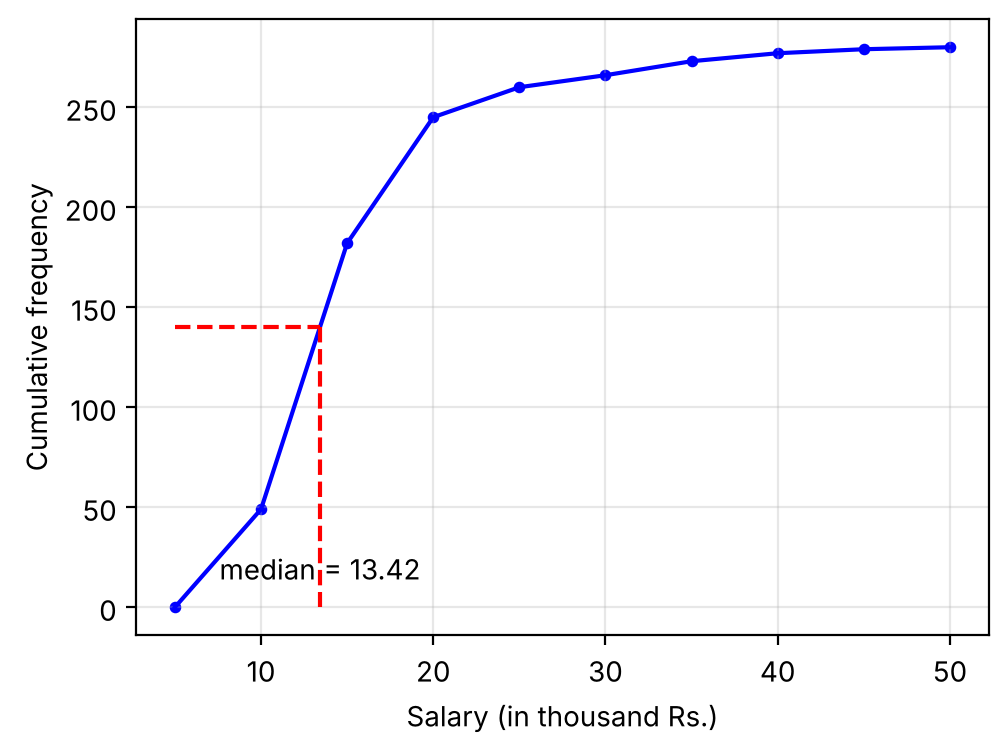
\includegraphics[width=0.70\linewidth]{figs/1.2.22.png}
    \caption{Less than type ogive for the salary data}
    \label{fig:median_q22}
\end{figure}

    \item 
    \begin{enumerate}[label=(\alph*), leftmargin=1.5em, labelsep=0.5em]
        \item A motor boat whose speed is $18\text{ km/h}$ in still water takes $1\text{ hour}$ more to go $24\text{ km}$ upstream than to return downstream to the same spot. Find the speed of the stream.
        
        \vspace{0.5em}
        \begin{center}
            \textbf{OR}
        \end{center}
        \vspace{0.5em}

        \item A train travels at a certain average speed for a distance of $63\text{ km}$ and then travels at a distance of $72\text{ km}$ at an average speed of $6\text{ km/h}$ more than its original speed. If it takes $3\text{ hours}$ to complete total journey, what is the original average speed?
    \end{enumerate}	\vspace{2pt}
    \noindent\textbf{(a) Solution:} Let the speed of the stream be $x\text{ km/h}$.

Given:
\begin{align}
    \text{Speed of boat in still water} &= 18\text{ km/h} \\
    \text{Speed upstream} &= (18 - x)\text{ km/h} \\
    \text{Speed downstream} &= (18 + x)\text{ km/h} \\
    \text{Distance} &= 24\text{ km}
\end{align}

Time taken upstream $t_1 = \frac{24}{18 - x}$ hours, and time taken downstream $t_2 = \frac{24}{18 + x}$ hours.

According to the given condition ($t_1 - t_2 = 1$ hour):
\begin{align}
    \frac{24}{18 - x} - \frac{24}{18 + x} &= 1 \\
    24 \left( \frac{(18 + x) - (18 - x)}{(18 - x)(18 + x)} \right) &= 1 \\
    24 \left( \frac{2x}{324 - x^2} \right) &= 1 \\
    48x &= 324 - x^2 \\
    &\implies x^2 + 48x - 324 = 0
\end{align}

Factoring the quadratic equation:
\begin{align}
    x^2 + 54x - 6x - 324 &= 0 \\
    x(x + 54) - 6(x + 54) &= 0 \\
    (x - 6)(x + 54) &= 0 \\
    &\implies x = 6 \quad \text{or} \quad x = -54
\end{align}

Since speed cannot be negative, $x = 6$.
Thus, the speed of the stream is $6\text{ km/h}$. \\[8pt]
\noindent\textbf{(b) Solution:} Let the original average speed of the train be $x\text{ km/h}$.

Given:
\begin{align}
    \text{Time for first 63 km} &= \frac{63}{x}\text{ hours} \\
    \text{Time for next 72 km} &= \frac{72}{x + 6}\text{ hours}
\end{align}

Total journey time is $3$ hours:
\begin{align}
    \frac{63}{x} + \frac{72}{x + 6} &= 3
\end{align}

Dividing the entire equation by 3:
\begin{align}
    \frac{21}{x} + \frac{24}{x + 6} &= 1 \\
    \frac{21(x + 6) + 24x}{x(x + 6)} &= 1 \\
    21x + 126 + 24x &= x^2 + 6x \\
    45x + 126 &= x^2 + 6x \\
    &\implies x^2 - 39x - 126 = 0
\end{align}

Factoring the quadratic equation:
\begin{align}
    x^2 - 42x + 3x - 126 &= 0 \\
    x(x - 42) + 3(x - 42) &= 0 \\
    (x - 42)(x + 3) &= 0 \\
    &\implies x = 42 \quad \text{or} \quad x = -3
\end{align}

Since speed cannot be negative, $x = 42$.
Thus, the original average speed of the train is $42\text{ km/h}$.The following code verifies both parts.
\begin{lstlisting}[frame=single, basicstyle=\rmfamily, escapeinside={(*@}{@*)}]
(*@\makebox[\dimexpr\linewidth-2\fboxsep-2\fboxrule\relax][c]{codes/1.2.23.py}@*)
\end{lstlisting}

    \item The sum of four consecutive numbers in an AP is 32 and the ratio of the product of the first and the last term to the product of two middle terms is $7 : 15$. Find the numbers.

\solution From \eqref{eq:EE26BTECH11225-ap-four}, let the four consecutive terms of the A.P. be $(a - 3d), (a - d), (a + d),$ and $(a + 3d)$. \\[2pt]
Given that the sum of these four numbers is 32:
\begin{align}
    (a - 3d) + (a - d) + (a + d) + (a + 3d) &= 32 \\
    &\implies 4a = 32 \\
    &\implies a = 8
\end{align}
Also given that the ratio of the product of the first and last terms to the product of the middle terms is $7 : 15$:
\begin{align}
    \frac{(a - 3d)(a + 3d)}{(a - d)(a + d)} &= \frac{7}{15} \\
    &\implies \frac{a^2 - 9d^2}{a^2 - d^2} = \frac{7}{15}
\end{align}
Substituting $a = 8$ ($a^2 = 64$):
\begin{align}
    \frac{64 - 9d^2}{64 - d^2} &= \frac{7}{15} \\
    &\implies 15(64 - 9d^2) = 7(64 - d^2) \\
    &\implies 960 - 135d^2 = 448 - 7d^2 \\
    &\implies 135d^2 - 7d^2 = 960 - 448 \\
    &\implies 128d^2 = 512 \\
    &\implies d^2 = \frac{512}{128} = 4 \\
    &\implies d = \pm 2
\end{align}
Taking $d = 2$:
\begin{align}
    a - 3d &= 8 - 3(2) = 2 \\
    a - d &= 8 - 2 = 6 \\
    a + d &= 8 + 2 = 10 \\
    a + 3d &= 8 + 3(2) = 14
\end{align}
(Taking $d = -2$ gives the same terms in reverse order: $14, 10, 6, 2$).

Thus, the four numbers are $2, 6, 10,$ and $14$.
    \item 
    \begin{enumerate}[label=(\alph*), leftmargin=1.5em, labelsep=0.5em]
        \item In an equilateral $\Delta ABC$, $D$ is a point on side $BC$ such that $BD = \frac{1}{3}BC$. Prove that $9(AD)^2 = 7(AB)^2$.
        
        \vspace{0.5em}
        \begin{center}
            \textbf{OR}
        \end{center}
        \vspace{0.5em}

        \item Prove that, in a right triangle, the square on the hypotenuse is equal to the sum of the squares on the other two sides.
    \end{enumerate}	\vspace{2pt}
    \noindent\textbf{(a) Solution:} Let $\Delta ABC$ be an equilateral triangle with side length $AB = BC = CA = a$.
Draw $AE \perp BC$. In an equilateral triangle, the altitude bisects the base, so:
\begin{align}
    BE = EC = \frac{a}{2}
\end{align}

Given $BD = \frac{1}{3}BC = \frac{a}{3}$.

Now, calculate $DE$:
\begin{align}
    DE &= BE - BD = \frac{a}{2} - \frac{a}{3} = \frac{a}{6}
\end{align}

In right $\Delta AEB$, by Pythagoras theorem, from \eqref{eq:EE26BTECH11225-pythagoras}:
\begin{align}
    AE^2 &= AB^2 - BE^2 = a^2 - \left(\frac{a}{2}\right)^2 = a^2 - \frac{a^2}{4} = \frac{3a^2}{4}
\end{align}

In right $\Delta AED$, by Pythagoras theorem, from \eqref{eq:EE26BTECH11225-pythagoras}:
\begin{align}
    AD^2 &= AE^2 + DE^2 \\
    AD^2 &= \frac{3a^2}{4} + \left(\frac{a}{6}\right)^2 \\
    AD^2 &= \frac{3a^2}{4} + \frac{a^2}{36} \\
    AD^2 &= \frac{27a^2 + a^2}{36} = \frac{28a^2}{36} = \frac{7a^2}{9} \\
    &\implies 9(AD)^2 = 7a^2
\end{align}

Since $a = AB$:
\begin{align}
    9(AD)^2 = 7(AB)^2
\end{align}
Hence proved. \\[8pt]
\noindent\textbf{(b) Solution:} Consider a right-angled triangle $ABC$, right-angled at $B$.

\textbf{To prove:} $AC^2 = AB^2 + BC^2$.

\textbf{Construction:} Draw $BD \perp AC$.

In $\Delta ADB$ and $\Delta ABC$:
\begin{align}
    \angle ADB &= \angle ABC = 90^\circ \\
    \angle A &= \angle A \quad \text{(Common angle)}
\end{align}
By AA similarity criterion, $\Delta ADB \sim \Delta ABC$.
Therefore, ratio of corresponding sides is equal:
\begin{align}
    \frac{AD}{AB} = \frac{AB}{AC} &\implies AB^2 = AD \times AC \label{eq:EE26BTECH11225-pyth-1}
\end{align}

In $\Delta BDC$ and $\Delta ABC$:
\begin{align}
    \angle BDC &= \angle ABC = 90^\circ \\
    \angle C &= \angle C \quad \text{(Common angle)}
\end{align}
By AA similarity criterion, $\Delta BDC \sim \Delta ABC$.
Therefore:
\begin{align}
    \frac{DC}{BC} = \frac{BC}{AC} &\implies BC^2 = DC \times AC \label{eq:EE26BTECH11225-pyth-2}
\end{align}

Adding \eqref{eq:EE26BTECH11225-pyth-1} and \eqref{eq:EE26BTECH11225-pyth-2}:
\begin{align}
    AB^2 + BC^2 &= (AD \times AC) + (DC \times AC) \\
    &= AC(AD + DC)
\end{align}

Since $AD + DC = AC$:
\begin{align}
    AB^2 + BC^2 &= AC \times AC = AC^2
\end{align}
Hence proved.
    
    \item Draw a triangle $ABC$ with $BC = 6\text{ cm}$, $AB = 5\text{ cm}$ and $\angle ABC = 60^\circ$. Then construct a triangle whose sides are $\frac{3}{4}$ of the corresponding sides of $\triangle ABC$.
\solution
Steps of construction:
\begin{enumerate}[label=(\roman*), leftmargin=1.5em, labelsep=0.5em]
    \item Draw $BC = 6\text{ cm}$.
    \item At $B$, draw ray $BY$ with $\angle CBY = 60^\circ$. With centre $B$ and radius $5\text{ cm}$, cut $BY$ at $A$. Join $AC$.
    \item Below $BC$, draw a ray $BX$ making an acute angle $\angle CBX$ with $BC$.
    \item Along $BX$, mark four points $B_1, B_2, B_3, B_4$ such that $BB_1 = B_1B_2 = B_2B_3 = B_3B_4$.
    \item Join $B_4C$. Through $B_3$, draw $B_3C' \parallel B_4C$ meeting $BC$ at $C'$.
    \item Through $C'$, draw $C'A' \parallel CA$ meeting $BA$ at $A'$.
\end{enumerate}
Then $\Delta A'BC'$ is the required triangle. \\
\textbf{Justification:} Since $B_3C' \parallel B_4C$, by the basic proportionality theorem
\begin{align}
    \frac{BC'}{BC} = \frac{BB_3}{BB_4} = \frac{3}{4}
\end{align}
Since $C'A' \parallel CA$, $\Delta A'BC' \sim \Delta ABC$, so
\begin{align}
    \frac{A'B}{AB} = \frac{BC'}{BC} = \frac{A'C'}{AC} = \frac{3}{4}
\end{align}
The following code verifies the construction and generates \figref{fig:construction_q26}.
\begin{lstlisting}[frame=single, basicstyle=\rmfamily, escapeinside={(*@}{@*)}]
(*@\makebox[\dimexpr\linewidth-2\fboxsep-2\fboxrule\relax][c]{codes/1.2.26.py}@*)
\end{lstlisting}
\begin{figure}[H]
    \centering
    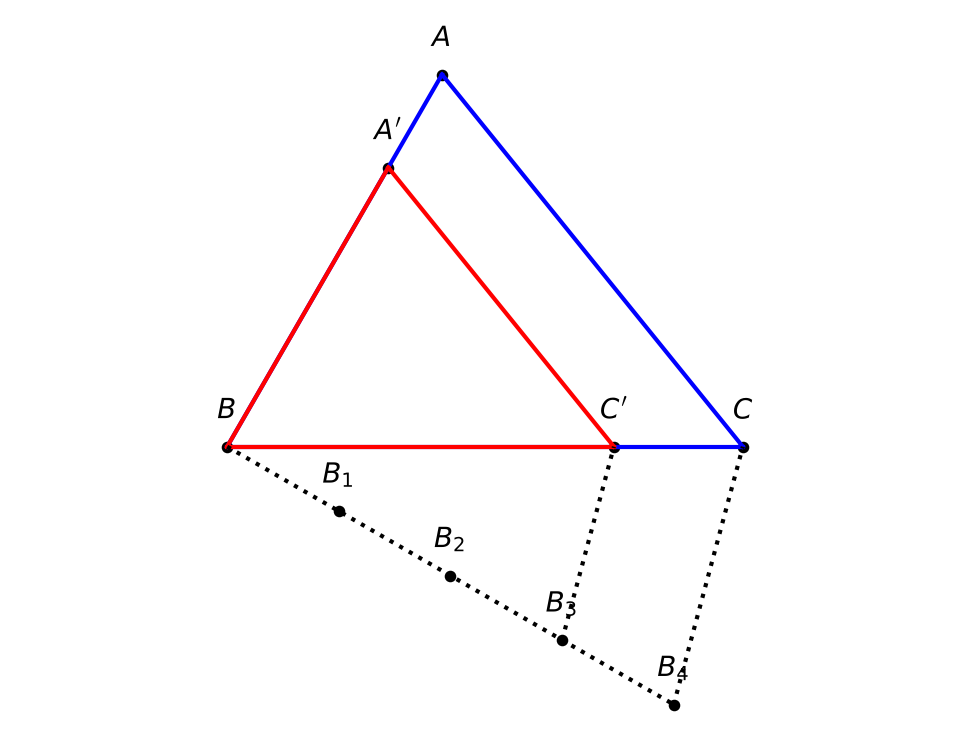
\includegraphics[width=0.75\linewidth]{figs/1.2.26.png}
    \caption{Construction of $\Delta A'BC'$}
    \label{fig:construction_q26}
\end{figure}

    \item Prove that:
    \[
    \frac{\sin A - 2\sin^3 A}{2\cos^3 A - \cos A} = \tan A.
    \]


\solution Taking the Left Hand Side (LHS):
\begin{align}
    \text{LHS} &= \frac{\sin A - 2\sin^3 A}{2\cos^3 A - \cos A} \\
    &= \frac{\sin A (1 - 2\sin^2 A)}{\cos A (2\cos^2 A - 1)}
\end{align}
From \eqref{eq:EE26BTECH11225-trig-1}, $\sin^2 A + \cos^2 A = 1 \implies 1 = \sin^2 A + \cos^2 A$:
\begin{align}
    1 - 2\sin^2 A &= (\sin^2 A + \cos^2 A) - 2\sin^2 A \\
    &= \cos^2 A - \sin^2 A \\
    2\cos^2 A - 1 &= 2\cos^2 A - (\sin^2 A + \cos^2 A) \\
    &= \cos^2 A - \sin^2 A
\end{align}
Substituting these into the expression:
\begin{align}
    \text{LHS} &= \frac{\sin A (\cos^2 A - \sin^2 A)}{\cos A (\cos^2 A - \sin^2 A)} \\
    &= \frac{\sin A}{\cos A} \\
    &= \tan A = \text{RHS}
\end{align}
Hence proved.The following code verifies the identity numerically and plots both sides in \figref{fig:identity_q27}.
\begin{lstlisting}[frame=single, basicstyle=\rmfamily, escapeinside={(*@}{@*)}]
(*@\makebox[\dimexpr\linewidth-2\fboxsep-2\fboxrule\relax][c]{codes/1.2.27.py}@*)
\end{lstlisting}
\begin{figure}[H]
    \centering
    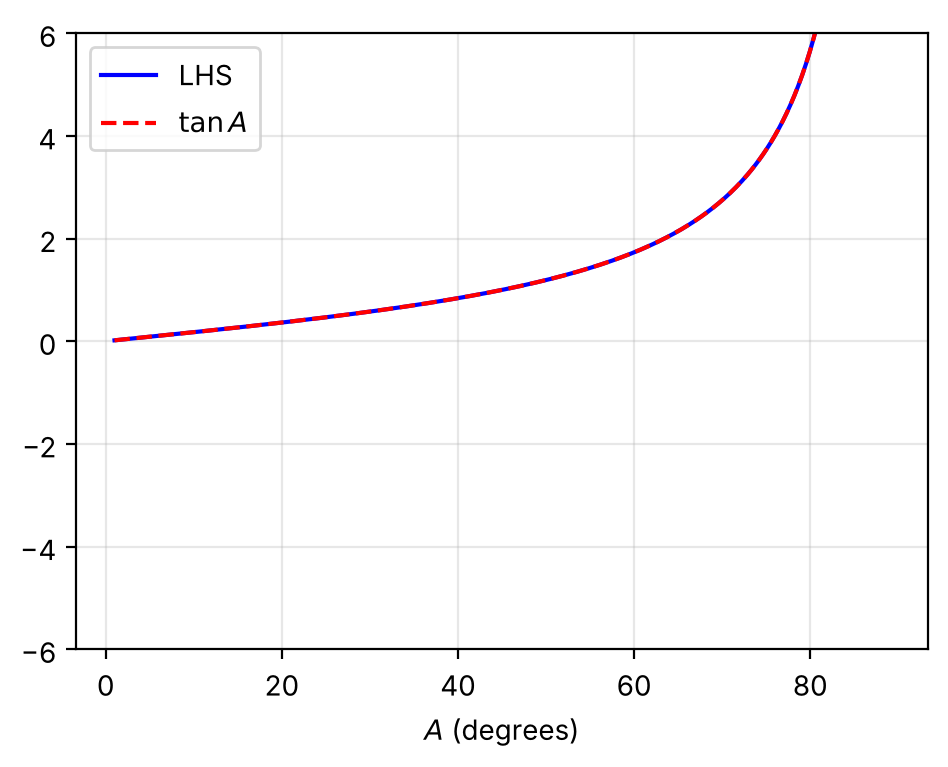
\includegraphics[width=0.70\linewidth]{figs/1.2.27.png}
    \caption{Plot of LHS and $\tan A$}
    \label{fig:identity_q27}
\end{figure}

    \item The diameters of the lower and upper ends of a bucket in the form of a frustum of a cone are 10 cm and 30 cm respectively. If its height is 24 cm, find:
\newline
    (i) The area of the metal sheet used to make the bucket.
\newline
    (ii) Why we should avoid the bucket made by ordinary plastic? [Use $\pi = 3.14$]

\solution Given:
Upper radius $R = \frac{30}{2} = 15\text{ cm}$, lower radius $r = \frac{10}{2} = 5\text{ cm}$, height $h = 24\text{ cm}$. \\[4pt]
From \eqref{eq:EE26BTECH11225-frustum-l}, the slant height $l$ of the frustum is:
\begin{align}
    l &= \sqrt{h^2 + (R - r)^2} \\
    &= \sqrt{24^2 + (15 - 5)^2} \\
    &= \sqrt{576 + 10^2} = \sqrt{576 + 100} = \sqrt{676} = 26\text{ cm}
\end{align}
(i) From \eqref{eq:EE26BTECH11225-frustum-area}, area of the metal sheet used = Curved Surface Area + Area of bottom circular base:
\begin{align}
    \text{Area} &= \pi(R + r)l + \pi r^2 \\
    &= \pi \left[ (15 + 5) \times 26 + 5^2 \right] \\
    &= \pi (20 \times 26 + 25) \\
    &= \pi (520 + 25) = 545 \pi \\
    &= 545 \times 3.14 = 1711.3\text{ cm}^2
\end{align}
Thus, the area of the metal sheet used is $1711.3\text{ cm}^2$. \\[6pt]
(ii) Plastic buckets should be avoided because ordinary plastic is non-biodegradable and causes environmental pollution. Additionally, plastics may leach toxic chemicals when stored with hot water or food items.
    \item As observed from the top of a 100 m high lighthouse from sea level, the angles of depression of two ships are $30^\circ$ and $45^\circ$. If one ship is exactly behind the other on the same side of the lighthouse, find the distance between the two ships. [Use $\sqrt{3} = 1.732$]

\solution Let $AB$ be the lighthouse of height $h = 100\text{ m}$, and $C, D$ be the two ships on the same side of the lighthouse such that the angles of depression are $45^\circ$ and $30^\circ$ respectively. Let $BC = x\text{ m}$ and $CD = y\text{ m}$ (the distance between the two ships).

\begin{center}
    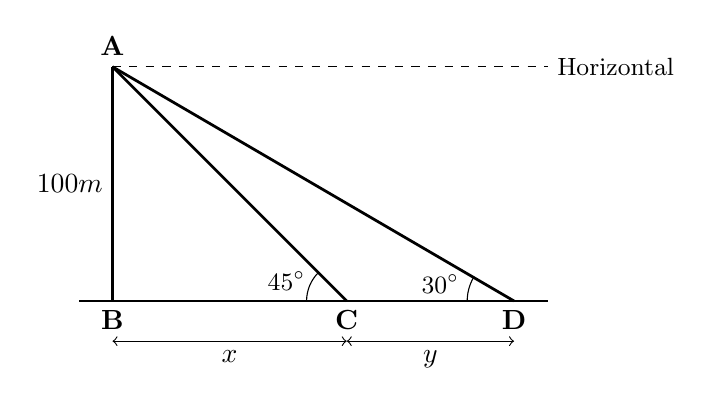
\begin{tikzpicture}[scale=0.85]
        % Horizontal ground/sea level
        \draw[thick] (-0.5,0) -- (6.5,0);
        
        % Lighthouse AB
        \draw[line width=1.2pt] (0,0) -- (0,3.5) node[above] {\textbf{A}};
        \node[below] at (0,0) {\textbf{B}};
        \node[left] at (0,1.75) {$100\text{ m}$};
        
        % Ships C and D
        \coordinate (C) at (3.5,0);
        \coordinate (D) at (6,0);
        \node[below] at (C) {\textbf{C}};
        \node[below] at (D) {\textbf{D}};
        
        % Lines of sight
        \draw[line width=1pt] (0,3.5) -- (3.5,0);
        \draw[line width=1pt] (0,3.5) -- (6,0);
        
        % Horizontal reference line at top for angles of depression
        \draw[dashed] (0,3.5) -- (6.5,3.5) node[right] {\small Horizontal};
        
        % Angles of elevation (alternate interior to angles of depression)
        \draw (2.9,0) arc (180:135:0.6);
        \node at (2.6,0.3) {\small $45^\circ$};
        
        \draw (5.3,0) arc (180:150:0.7);
        \node at (4.9,0.25) {\small $30^\circ$};
        
        % Distance labels
        \draw[<->] (0,-0.6) -- (3.5,-0.6) node[midway,below] {$x$};
        \draw[<->] (3.5,-0.6) -- (6,-0.6) node[midway,below] {$y$};
    \end{tikzpicture}

    \captionof{figure}{Lighthouse $AB$ with ships $C$ and $D$}
    \label{fig:lighthouse_q29}
\end{center}

In right triangle $\Delta ABC$, from \eqref{eq:EE26BTECH11225-trig-ratios}:
\begin{align}
    \tan 45^\circ &= \frac{AB}{BC} \\
    &\implies 1 = \frac{100}{x} \\
    &\implies x = 100\text{ m}
\end{align}

In right triangle $\Delta ABD$, from \eqref{eq:EE26BTECH11225-trig-ratios}:
\begin{align}
    \tan 30^\circ &= \frac{AB}{BD} = \frac{AB}{x + y} \\
    &\implies \frac{1}{\sqrt{3}} = \frac{100}{100 + y} \\
    &\implies 100 + y = 100\sqrt{3} \\
    &\implies y = 100\sqrt{3} - 100 \\
    &\implies y = 100(\sqrt{3} - 1) \\
    &\implies y = 100(1.732 - 1) = 100(0.732) = 73.2\text{ m}
\end{align}
Thus, the distance between the two ships is $73.2\text{ m}$.
    \item 
    \begin{enumerate}[label=(\alph*), leftmargin=1.5em, labelsep=0.5em]
    		\item The mean of the following distribution is $18$. Find the frequency $f$ of the class $19\text{--}21$.
    
    \begin{center}
    \begin{tabular}{|c|c|c|c|c|c|c|c|}
        \hline
        \textbf{Class} & 11--13 & 13--15 & 15--17 & 17--19 & 19--21 & 21--23 & 23--25 \\ \hline
        \textbf{Frequency} & 3 & 6 & 9 & 13 & $f$ & 5 & 4 \\ \hline
    \end{tabular}
    \end{center}
        
        \vspace{0.5em}
        \begin{center}
            \textbf{OR}
        \end{center}
        \vspace{0.5em}

        \item The following distribution gives the daily income of $50$ workers of a factory:

\begin{center}
\begin{tabular}{|c|c|c|c|c|c|}
    \hline
    \textbf{Daily Income (in Rs.)} & 100--120 & 120--140 & 140--160 & 160--180 & 180--200 \\ \hline
    \textbf{Number of workers} & 12 & 14 & 8 & 6 & 10 \\ \hline
\end{tabular}
\end{center}

Convert the distribution above to a less than type cumulative frequency distribution and draw its ogive.
    \end{enumerate}	\vspace{2pt}
    \noindent\textbf{(a) Solution:} Constructing the frequency table to calculate the mean:

\begin{center}
\begin{tabular}{|c|c|c|c|}
    \hline
    \textbf{Class Interval} & \textbf{Class Mark ($x_i$)} & \textbf{Frequency ($f_i$)} & \textbf{$f_i x_i$} \\
    \hline
    11--13 & 12 & 3 & 36 \\
    13--15 & 14 & 6 & 84 \\
    15--17 & 16 & 9 & 144 \\
    17--19 & 18 & 13 & 234 \\
    19--21 & 20 & $f$ & $20f$ \\
    21--23 & 22 & 5 & 110 \\
    23--25 & 24 & 4 & 96 \\
    \hline
    \textbf{Total} & & $\sum f_i = 40 + f$ & $\sum f_i x_i = 704 + 20f$ \\
    \hline
\end{tabular}
\end{center}

Given Mean ($\bar{x}$) $= 18$. From \eqref{eq:EE26BTECH11225-mean}, the mean is:
\begin{align}
    \bar{x} &= \frac{\sum f_i x_i}{\sum f_i} \\
    18 &= \frac{704 + 20f}{40 + f} \\
    18(40 + f) &= 704 + 20f \\
    720 + 18f &= 704 + 20f \\
    720 - 704 &= 20f - 18f \\
    16 &= 2f \\
    &\implies f = \frac{16}{2} = 8
\end{align}
Thus, the missing frequency $f$ is $8$. \\[8pt]
\noindent\textbf{(b) Solution:} Converting the given data into a ``less than type'' cumulative frequency distribution:

\begin{center}
\begin{tabular}{|c|c|}
    \hline
    \textbf{Daily Income (in Rs.)} & \textbf{Cumulative Frequency (cf)} \\
    \hline
    Less than 120 & 12 \\
    Less than 140 & 26 \quad ($12 + 14$) \\
    Less than 160 & 34 \quad ($26 + 8$) \\
    Less than 180 & 40 \quad ($34 + 6$) \\
    Less than 200 & 50 \quad ($40 + 10$) \\
    \hline
\end{tabular}
\end{center}

To plot the ``less than type'' ogive, plot the points $(100, 0)$ (the lower limit of the first class, where the cumulative frequency is $0$), $(120, 12)$, $(140, 26)$, $(160, 34)$, $(180, 40)$, and $(200, 50)$ on a graph with upper limits on the $x$-axis and cumulative frequencies on the $y$-axis, and join them with a smooth freehand curve. The following code verifies part (a) and plots the ogive in \figref{fig:ogive_q30}.

\begin{lstlisting}[frame=single, basicstyle=\rmfamily, escapeinside={(*@}{@*)}]
(*@\makebox[\dimexpr\linewidth-2\fboxsep-2\fboxrule\relax][c]{codes/1.2.30.py}@*)
\end{lstlisting}
\begin{figure}[H]
    \centering
    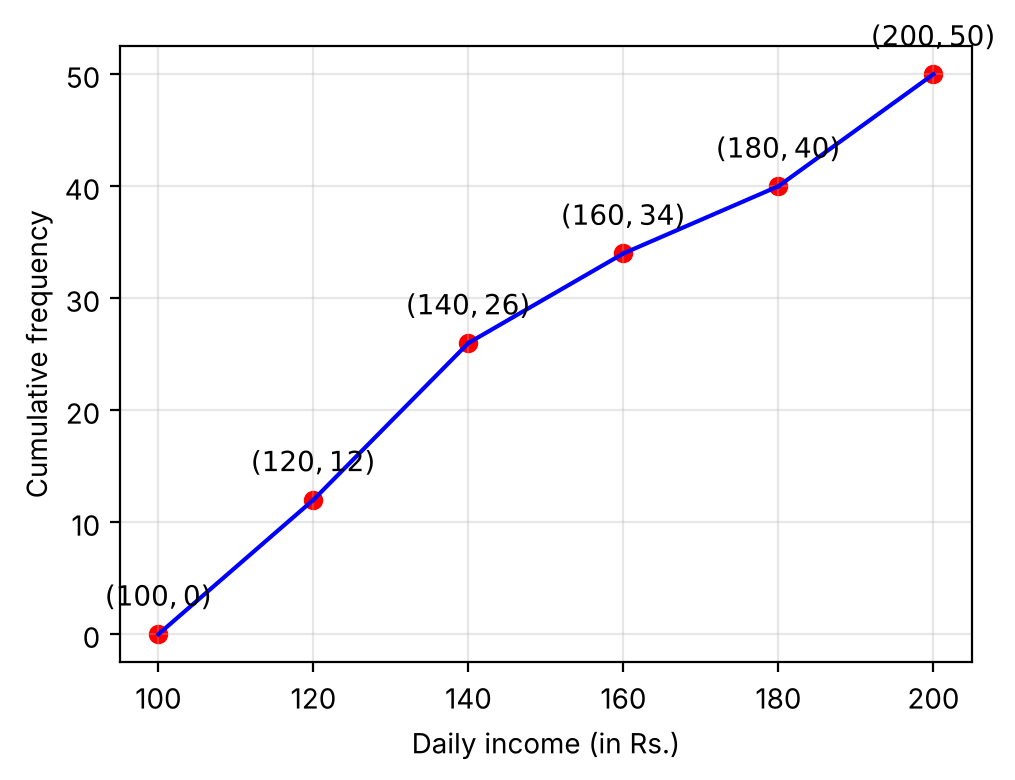
\includegraphics[width=0.70\linewidth]{figs/1.2.30.png}
    \caption{Less than type ogive for daily income distribution}
    \label{fig:ogive_q30}
\end{figure}
\end{enumerate}
